\renewcommand{\sectionauthor}{Prof. Gustavo Ale}

\begin{multicols*}{2}

    \section*{Geometria}
    A geometria é provavelmente a área mais antiga da matemática, precursora da própria álgebra e sendo um dos pilares
    da matemática. A palavra geometria é resultado da combinação das palavras gregas \textit{geo} e
    \textit{metron}/\textit{metri}, significando respectivamente Terra e medição, pois a área da geometria consiste da
    medição e entendimento das relações e propriedades  contidas nas fíguras geométricas: comprimento, distância, ângulo,
    área, volume e perímetro, as fíguras geométricas por sua vez são parte integrante da natureza e da Terra (\textit{geo}).

    \subsection*{Definições gerais}
    Antes do estudo da geometria devemos ter ciência das definições de conceitos presentes nesse ramo da matemática,
    dentro destes conceitos se enquadram as medidas, os ângulos, as fíguras geométricas e suas componentes.

    \vfill\null
    \columnbreak
    \vfill\null

    \subsection*{Grandezas e unidades de medida}
    \subsubsection*{Distância e comprimento}
    Distância e comprimento medem o quão longe dois pontos estão entre si, e no caso de arestas essa medida é
    denotada como comprimento. A unidade de medida base utilizada para comprimento é o metro (símbolo ${m}$), além do
    metro existem seus múltiplos que são igualmente utilizados dependendo da distância/comprimento aferido.

    \begin{figure}[H]
        \centering
        %\resizebox{\columnwidth}{!}
        \caption{$d$ representa a distância entre os pontos que formam a reta $\overline{AB}$}
    \end{figure}

    \begin{table}[H]
        \resizebox{\columnwidth}{!}{%
            \begin{tabular}{l|l|l}
                \rowcolor{gray!25}
                \textbf{Nome} & \textbf{Sigla} & \textbf{Equivalência} \\ \hline
                picômetro     & $pm$           & $10^{-12}m$           \\ \rowcolor{gray!10}
                nanometro     & $nm$           & $10^{-9}m$            \\
                micrometro    & $\mu m$        & $10^{-6}m$            \\ \rowcolor{gray!10}
                milimetro     & $mm$           & $10^{-3}m$            \\
                centímetro    & $cm$           & $10^{-2}m$            \\ \rowcolor{gray!10}
                decímetro     & $dm$           & $10^{-1}m$            \\
                metro         & $m$            & $1m$                  \\ \rowcolor{gray!10}
                decâmetro     & $dam$          & $10m$                 \\
                hêctometro    & $hm$           & $100m$                \\ \rowcolor{gray!10}
                quilometro    & $km$           & $1000m$
            \end{tabular}%
        }
        %\caption{Unidades medida de comprimento e distância}
    \end{table}
    Outras medidas de comprimento são: \\
    \textbf{Perímetro:} comprimento do contorno de uma fígura geométrica. \\
    \textbf{Raio:} distância entre o centro de uma circunferência até seu contorno ou superfície.\\
    \textbf{Diâmetro:} comprimento de reta que passe pelo centro da circunferência e cujo seus pontos de
    início e fim estejam sobre a circunferência\\
    \textbf{Circunferência:} perímetro de uma circunferência.\\

    \begin{figure}[H]
        \centering
        %\resizebox{\columnwidth}{!}{%
        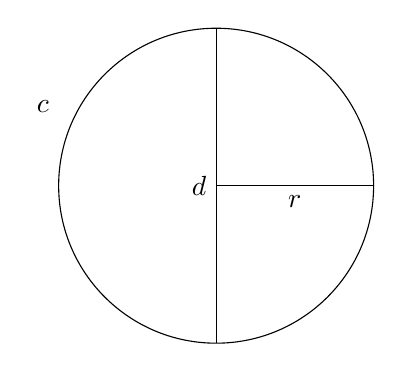
\begin{tikzpicture}
            \coordinate (A) at (2,2);
            \coordinate (B) at (4,2);
            \coordinate (C) at (2,0);
            \coordinate (D) at (2,4);
            \draw (A)--node[below] {$r$}(B) ;
            \draw (C)--node[left] {$d$}(D) ;
            \draw (A) circle (2cm)
            (0,3) node[left] {$c$};
        \end{tikzpicture}
        %}
        \caption{Raio $r$, diâmetro $d$ e circunferência $c$ de um círculo}
    \end{figure}

    o diâmetro de um círculo é $d = 2r$, logo o raio é $r = \frac{d}{2}$ e a circunferência/perímetro do círculo é $2\pi r$.
    Onde $\pi$ é a constante matemática \textit{pi}, cujo valor é aproximadamente $3.14159265...$

    % \begin{figure}[H]
    %     \centering
    %     
\includegraphics[width=0.7\columnwidth]{assets/image_placeholder.png}
    %     \caption{Raio, diâmetro e circunferência de um círculo}
    % \end{figure}

    \subsubsection*{Área}
    Área é a medida que expressa a quantidade de espaço bidimensional ocupado por uma fígura geométrica,
    área de superfície é o equivalente da área para uma superfície ou face de um objeto tridimensional. A unidade base
    para área é o metro quadrado (símbolo ${m^2}$). Seus múltiplos também acompanham o termo 'quadrado',
    e a equivalência é a mesma do metro, porém elevada ao quadrado. Ex.: $1m = 10^2cm$ e $1m^2 = (10^2cm)^2 = 10^4cm^2$,
    lembrar essa regra pode facilitar na hora da conversão de área.

    \begin{figure}[H]
        \centering
        %\resizebox{\columnwidth}{!}{%
        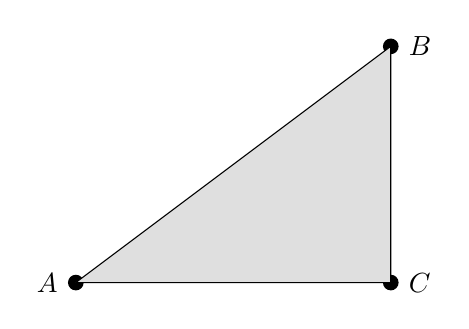
\begin{tikzpicture}
            \coordinate (A) at (0,0);
            \coordinate (B) at (4,3);
            \coordinate (C) at (4,0);
            % \coordinate (D) at (0,3);
            \node[circle, fill, label={left:$A$}, inner sep=2pt] at (A) {};
            \node[circle, fill, label={right:$B$}, inner sep=2pt] at (B) {};
            \node[circle, fill, label={right:$C$}, inner sep=2pt] at (C) {};
            % \node[circle, fill, label={left:$D$}, inner sep=2pt] at (D) {};
            % \draw[dashed] (A)--(D)--(B);
            \draw[fill=gray!25] (A)--(B)--(C)--(A);
        \end{tikzpicture}
        %}
        \caption{Área é o espaço bidimensional ocupado pela região cinza.}
        \label{fig:tri_abc}
    \end{figure}

    \begin{table}[H]
        \resizebox{\columnwidth}{!}{%
            \begin{tabular}{l|l|l}
                \rowcolor{gray!25}
                \textbf{Nome}       & \textbf{Sigla} & \textbf{Equivalência}       \\ \hline
                picômetro quadrado  & $pm^2$         & $10^{-24}m^2$               \\ \rowcolor{gray!10}
                nanometro quadrado  & $nm^2$         & $10^{-18}m^2$               \\
                micrometro quadrado & $\mu m$        & $10^{-12}m^2$               \\ \rowcolor{gray!10}
                milimetro quadrado  & $mm^2$         & $10^{-6}m^2$                \\
                centímetro quadrado & $cm^2$         & $10^{-4}m^2$                \\ \rowcolor{gray!10}
                decímetro quadrado  & $dm^2$         & $10^{-2}m^2$                \\
                metro quadrado      & $m^2$          & $1m^2$                      \\ \rowcolor{gray!10}
                decâmetro quadrado  & $dam^2$        &                             \\ \rowcolor{gray!10}
                are                 & $are$          & \multirow{-2}{*}{$100m^2$}  \\
                hêctometro quadrado & $hm^2$         &                             \\
                hectare             & $ha$           & \multirow{-2}{*}{$10^4m^2$} \\ \rowcolor{gray!10}
                quilometro quadrado & $km^2$         & $10^6m^2$
            \end{tabular}%
        }
        %\caption{Unidades medida de área}
    \end{table}

    \subsubsection*{Volume}
    Assim como a área expressa a quantidade de espaço bidimensional ocupado por uma fígura geométrica, o volume expressa
    a quantidade de espaço tridimensional ocupado por um objeto. No caso do volume existe duas unidades de medida base,
    o metro cúbico e o litro, ambos são usados regularmente, na qual o litro é a unidade mais usada para volumes
    pequenos, enquanto o metro cúbico é usado para expressar volumes maiores.

    \begin{figure}[H]
        \centering
        %\resizebox{0.5\columnwidth}{!}{%
        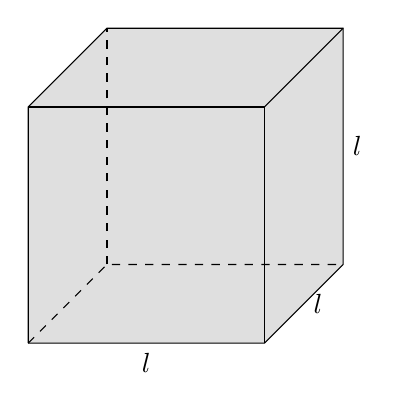
\begin{tikzpicture}
            \coordinate (A) at (0,0);
            \coordinate (B) at (0,3);
            \coordinate (C) at (3,3);
            \coordinate (D) at (3,0);
            \coordinate (E) at (1,1);
            \coordinate (F) at (1,4);
            \coordinate (G) at (4,4);
            \coordinate (H) at (4,1);
            \draw[fill=gray!25] (A)--(B)--(F)--(G)--node[right]{$l$}(H)--node[right]{$l$}(D)--node[below]{$l$}(A);
            \draw (B)--(C)--(D);
            \draw (C)--(G);
            \draw[dashed] (A)--(E)--(H);
            \draw[dashed] (E)--(F);
        \end{tikzpicture}
        %}
        \caption{Cubo, cujo volume se dá por $l^3$, onde $l$ é o comprimento das arestas}
    \end{figure}

    \begin{table}[H]
        \resizebox{\columnwidth}{!}{%
            \begin{tabular}{l|l|l}
                \rowcolor{gray!25}
                \textbf{Nome}     & \textbf{Sigla} & \textbf{Equivalência}          \\ \hline
                milimetro cúbico  & $mm^3$         & $10^{-9}m^3$                   \\ \rowcolor{gray!10}
                centímetro cúbico & $cm^3$         &                                \\ \rowcolor{gray!10}
                mililitro         & $ml$           & \multirow{-2}{*}{$10^{-6}m^3$} \\
                decímetro cúbico  & $dm^3$         &                                \\ %\hline
                litro             & $l$            & \multirow{-2}{*}{$10^{-3}m^3$} \\ \rowcolor{gray!10}
                metro cúbico      & $m^3$          & $1m^2$                         \\ %\hline                      
            \end{tabular}%
        }
        %\caption{Unidades medida de volume}
    \end{table}

    \subsubsection*{Ângulo}

    Ângulo é uma medida de inclinação entre duas retas ou dois planos, desde que eles não sejam paralelos entre si, no
    contexto da geometria os ângulos estão presentes em todos os vértices das fíguras geométricas.
    As unidades de medida mais comuns para ângulo são graus (símbolo $^{\circ}$), radianos (símbolo $rad$) e gradianos (símbolo $gon$).

    Quanto no escopo das funções trigonométricas a unidade de medida mais utilizada é o radiano, por outro lado,
    em aplicações de engenharia e na geometria a unidade mais usada é o grau. Considerando um grau $\alpha$ em graus,
    sua conversão para radianos se dá por $rad(\alpha) = \alpha\cdot\pi/180$

    \begin{figure}[H]
        \centering
        %\resizebox{\columnwidth}{!}{%
        \begin{tikzpicture}
            \coordinate (O) at (1,2);
            \coordinate (A) at (0.5,1);
            \coordinate (B) at (2.5,5);
            \coordinate (C) at (0,2);
            \coordinate (D) at (5,2);
            \draw (A)--(B) node[above] {$p$}  ;
            \draw (C)--(D) node[above] {$q$};
            % \pic[angle radius=1cm,"$\alpha$"] {angle=a--b--c};
            \pic ["$65^{\circ}$", draw, -, angle eccentricity=2] {angle = D--O--B};
            % \draw (B)--(C);
            % \draw (A)--(C);
        \end{tikzpicture}
        %}
        \caption{Ângulo entre as retas $p$ e $q$}
    \end{figure}

    O ângulo apresenta uma importância muito grande no desenvolvimento da geometria e dos problemas geométricos, sendo o
    ângulo uma grandeza imprescindível no desenrolar da matemática entorno das fíguras geométricas, principalmente os
    triângulos.

    \subsection*{Fíguras geométricas e suas componentes}

    \subsubsection*{Ponto}
    A primeira componente das fíguras geométricas e a mais simples delas é o ponto, o mesmo deve ser imaginado como um
    ponto infinitesimal, não possuindo comprimento, área ou perímetro. Quando um ponto é integrante de uma fígura
    geométrica o mais comum é chamarmos ele de \textit{vértice}
    \begin{figure}[H]
        \centering
        %\resizebox{\columnwidth}{!}{%
        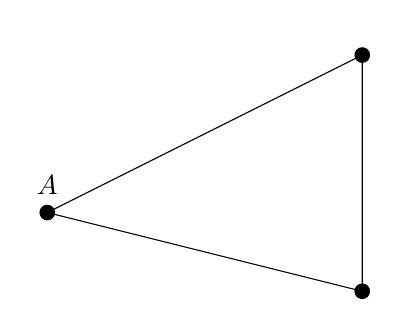
\begin{tikzpicture}
            \coordinate (A) at (1,1);
            \coordinate (B) at (5,3);
            \coordinate (C) at (5,0);
            \node[circle, fill, label={above:$A$}, inner sep=2pt] at (A) {};
            \node[circle, fill, label=, inner sep=2pt] at (B) {};
            \node[circle, fill, label=, inner sep=2pt] at (C) {};
            \draw (A)--(B)--(C)--(A);
        \end{tikzpicture}
        %}
        \caption{Triângulo com o vértice $A$ em realce }
        % \label{fig:vertice_tri}
    \end{figure}


    % \begin{figure}[H]
    %     \centering
    %     
\includegraphics[width=0.7\columnwidth]{assets/image_placeholder.png}
    %     \caption{Vértice de um triângulo }
    % \end{figure}

    A partir de dois pontos $A$ e $B$ podemos traçar uma reta $\overline{AB}$ entre eles e caso exista um terceiro ponto $C$ sob a mesma reta,
    então esses três pontos são \textbf{colineares}.

    \begin{figure}[H]
        \centering
        %\resizebox{\columnwidth}{!}
        \caption{Pontos colineares $A$,$B$ e $C$}
        \label{fig:reta_ab}
    \end{figure}

    % \begin{figure}[H]
    %     \centering
    %     
\includegraphics[width=0.7\columnwidth]{assets/image_placeholder.png}
    %     \caption{Pontos colineares}
    %     \label{fig:reta_abc}
    % \end{figure}

    \subsubsection*{Reta}
    A reta é um conjunto de pelo menos dois pontos, no caso dois pontos quaisquer $A$ e $B$ podem gerar a reta $\overline{AB}$, como na fígura \ref{fig:reta_ab}.
    Assim como o ponto é idealmente infinitesimal a reta idealmente não possui espessura. Quando uma reta é parte
    integrante de uma fígura geométrica sua denominação é \textit{aresta}.

    \begin{figure}[H]
        \centering
        %\resizebox{\columnwidth}{!}{%
        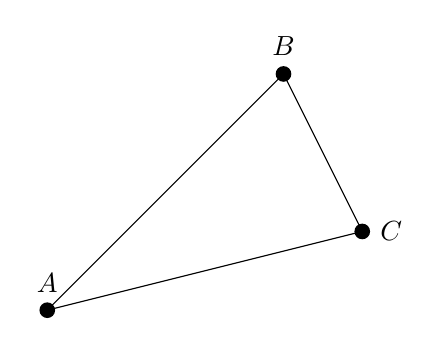
\begin{tikzpicture}
            \coordinate (A) at (0,0);
            \coordinate (B) at (3,3);
            \coordinate (C) at (4,1);
            \node[circle, fill, label={above:$A$}, inner sep=2pt] at (A) {};
            \node[circle, fill, label={above:$B$}, inner sep=2pt] at (B) {};
            \node[circle, fill, label={right:$C$}, inner sep=2pt] at (C) {};
            \draw (A)--(B)--(C)--(A);
        \end{tikzpicture}
        %}
        \caption{Retas $\overline{AB}$,$\overline{BC}$ e $\overline{AC}$ do triângulo $ABC$}
        \label{fig:tri_abc}
    \end{figure}

    % \begin{figure}[H]
    %     \centering
    %     
\includegraphics[width=0.7\columnwidth]{assets/image_placeholder.png}
    %     \caption{Reta $\overline{AB}$ do triângulo $\overline{ABC}$}
    %     \label{fig:reta_ab}
    % \end{figure}

    Uma reta $p$ é \textbf{perpendicular} a reta $q$ se o ângulo formado entre elas for de 90 graus.

    \begin{figure}[H]
        \centering
        %\resizebox{\columnwidth}{!}{%
        \begin{tikzpicture}
            \coordinate (O) at (1,1.5);
            \coordinate (A) at (0,2);
            \coordinate (B) at (4,0);
            \coordinate (C) at (0,0);
            \coordinate (D) at (3,4.5);
            \draw (A)--(B) node[above] {$p$}  ;
            \draw (C)--(D) node[left] {$q$};
            % \pic[angle radius=1cm,"$\alpha$"] {angle=a--b--c};
            \pic ["$90^{\circ}$", draw, -, angle eccentricity=2] {angle = B--O--D};
            % \draw (B)--(C);
            % \draw (A)--(C);
        \end{tikzpicture}
        %}
        \caption{Retas perpendiculares $p$ e $q$}
    \end{figure}

    % \begin{figure}[H]
    %     \centering
    %     
\includegraphics[width=0.7\columnwidth]{assets/image_placeholder.png}
    %     \caption{Retas perpendiculares $p$ e $q$}
    % \end{figure}

    %\columnbreak
    Duas retas $p$ e $q$ são consideradas \textbf{paralelas entre si}, se qualquer reta $r$ perpendicular a reta $p$ também for
    perpendicular a reta $q$. Outra forma de descrever retas paralelas é através do \textbf{Quinto Postulado de Euclides}
    que diz: Supondo que duas retas $p$ e $q$ são cortadas por uma terceira reta $r$. Se a soma dos ângulos formados um
    mesmo lado da reta $r$ resultar em 180 graus, então $m$ e $n$ são retas paralelas entre si.

    \begin{figure}[H]
        \centering
        %\resizebox{\columnwidth}{!}
        \caption{Retas paralelas $p$ e $q$}
    \end{figure}

    % \begin{figure}[H]
    %     \centering
    %     
\includegraphics[width=0.7\columnwidth]{assets/image_placeholder.png}
    %     \caption{Retas paralelas $p$ e $q$}
    % \end{figure}


    \subsubsection*{Plano e superfície}
    Quando se tem 3 ou mais pontos o resultado da conexão deles é tido como superfície, plano ou fígura geométrica
    dependendo da área da matemática e do contexto de estudo, porém vale ter em mente que também existem superfícies
    não bidimensionais. Uma exceção a isso são os círculos e as elipses que não possuem vértices. No contexto da
    geometria a ser estudado nesse capítulo a conexão de 3 ou mais vértices geram exclusivamente fíguras geométricas.

    \begin{figure}[H]
        \centering
        %\resizebox{\columnwidth}{!}{%
        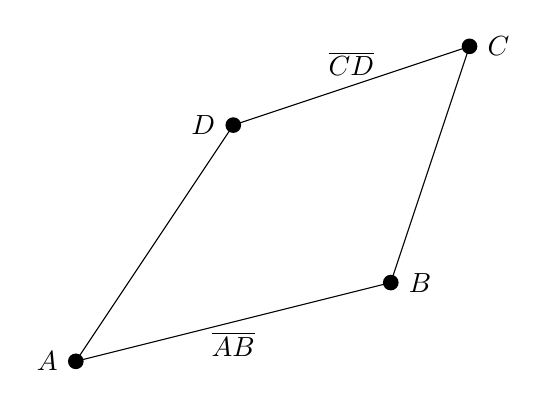
\begin{tikzpicture}
            \coordinate (A) at (0,0);
            \coordinate (B) at (4,1);
            \coordinate (C) at (5,4);
            \coordinate (D) at (2,3);
            \draw (A)-- node[below] {$\overline{AB}$} (B) ;
            \draw (B)--(C) ;
            \draw (C)-- node[above] {$\overline{CD}$} (D) ;
            \draw (D)--(A) ;
            \node[circle, fill, label={left:$A$}, inner sep=2pt] at (A) {};
            \node[circle, fill, label={right:$B$}, inner sep=2pt] at (B) {};
            \node[circle, fill, label={right:$C$}, inner sep=2pt] at (C) {};
            \node[circle, fill, label={left:$D$}, inner sep=2pt] at (D) {};
        \end{tikzpicture}
        %}
        \caption{Um quadrilátero $ABCD$ com as arestas $\overline{AB}$ e $\overline{CD}$ realçadas}
    \end{figure}

    % \begin{figure}[H]
    %     \centering
    %     
\includegraphics[width=0.7\columnwidth]{assets/image_placeholder.png}
    %     \caption{Um quadrilátero com as arestas realçadas em vermelho}
    % \end{figure}

    \subsubsection*{Sólidos}
    No contexto de fíguras geométricas tridimensionais, ou chamados sólidos, os sólidos podem ser formados por 4 ou
    mais pontos ou através manipulação de fíguras geométricas bidimensionais num espaço tridimensional.
    Todos objetos físicos que conhecemos podem ser abstraídos como formas geométricas, independente da complexidade.

    %\columnbreak
    Grandezas notórias das componentes citadas:
    \begin{itemize}
        \setlength\itemsep{1.15pt}
        \item Ponto, vértice: distância relativo a outro objeto.
        \item Reta: comprimento, distância e ângulo relativos a outro objeto.
        \item Superfície: área, perímetro.
        \item Sólido: volume.
    \end{itemize}

    \begin{figure}[H]
        \centering
        %\resizebox{\columnwidth}{!}{%
        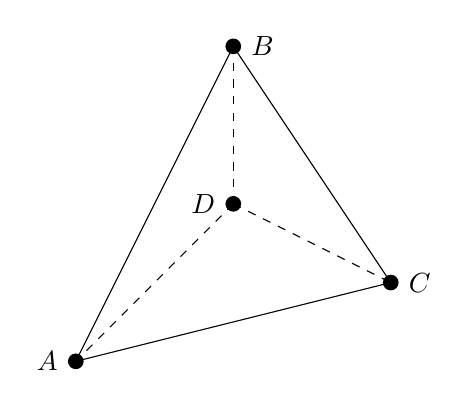
\begin{tikzpicture}
            \coordinate (A) at (0,0);
            \coordinate (B) at (2,4);
            \coordinate (C) at (4,1);
            \coordinate (D) at (2,2);
            \draw (A)--(B) ;
            \draw (B)--(C) ;
            \draw (C)--(A) ;
            \draw[dashed] (D)--(A) ;
            \draw[dashed] (D)--(B) ;
            \draw[dashed] (D)--(C) ;
            \node[circle, fill, label={left:$A$}, inner sep=2pt] at (A) {};
            \node[circle, fill, label={right:$B$}, inner sep=2pt] at (B) {};
            \node[circle, fill, label={right:$C$}, inner sep=2pt] at (C) {};
            \node[circle, fill, label={left:$D$}, inner sep=2pt] at (D) {};
        \end{tikzpicture}
        %}
        \caption{Tetraedro, o objeto tridimensional com menos faces}
    \end{figure}



\end{multicols*}

\section*{Área e volume}
% \subsection*{Fíguras planas}
\begin{table}[H]
    \setlength{\tabcolsep}{5mm} % separator between columns
    \def\arraystretch{2} % vertical stretch factor
    \newcommand{\tikzsize}{0.25\columnwidth/10cm}
    \centering
    \caption{Área de fíguras planas comuns}
    \resizebox{\textwidth}{!}{%
        \begin{tabular}{c|c|c|c}
            \rowcolor{gray!25}
            \multicolumn{2}{c|}{\textbf{Figura}}     & \textbf{Área} & \textbf{Perímetro}         \\ \hline
            Triângulo retângulo &    
            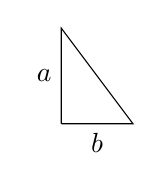
\begin{tikzpicture}[baseline=(current bounding box.center),scale=\tikzsize]
                    \coordinate (A) at (0,0);
                    \coordinate (B) at (0,4);
                    \coordinate (C) at (3,0);
                    \coordinate (D) at (0,2);
                    \draw (A)-- node[left]{$a$} (B)--(C)-- node[below]{$b$}(A);
                    \addvmargin{2mm};
                \end{tikzpicture}  
            & $\displaystyle \frac{a\cdot b}{2}$ &  $a+b+\sqrt{a^2+b^2}$   \\ \hline
            Triângulo equilátero & 
            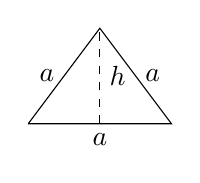
\begin{tikzpicture}[baseline=(current bounding box.center),scale=\tikzsize]
                \coordinate (A) at (-3,0);
                \coordinate (B) at (0,4);
                \coordinate (C) at (3,0);
                \coordinate (D) at (0,0);
                \draw (A)-- node[left]{$a$} (B)--node[right]{$a$}(C)-- node[below]{$a$}(A);
                \draw[dashed] (D) -- node[right] {$h$} (B);
                \addvmargin{2mm};
            \end{tikzpicture}  
            & $\displaystyle \frac{a\cdot h}{2}$ ou $\displaystyle \frac{h^2}{\sqrt{3}}$ ou $\displaystyle \frac{\sqrt{3}}{4}a^2$  &  $3a$    \\ \hline
            Triângulo isósceles &
            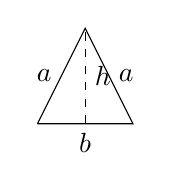
\begin{tikzpicture}[baseline=(current bounding box.center),scale=\tikzsize]
                \coordinate (A) at (-2,0);
                \coordinate (B) at (0,4);
                \coordinate (C) at (2,0);
                \coordinate (D) at (0,0);
                \draw (A)-- node[left]{$a$} (B)--node[right]{$a$}(C)-- node[below]{$b$}(A);
                \draw[dashed] (D) -- node[right] {$h$} (B);
                \addvmargin{2mm};
            \end{tikzpicture}  
            & $\displaystyle \frac{b\cdot h}{2}$  & $2a+b$       \\ \hline
            Retângulo  & 
            \begin{tikzpicture}[baseline=(current bounding box.center),scale=\tikzsize]
                \coordinate (A) at (0,0);
                \coordinate (B) at (0,3);
                \coordinate (C) at (4,3);
                \coordinate (D) at (4,0);
                \draw (A)-- node[left]{$a$} (B) -- (C) -- (D) -- node[below] {$b$} (A);
                \addvmargin{2mm};
            \end{tikzpicture} 
            & $a\cdot b$  & $2(a+b)$      \\ \hline
            Paralelogramo & 
            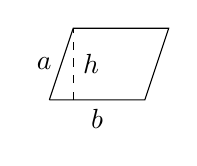
\begin{tikzpicture}[baseline=(current bounding box.center),scale=\tikzsize]
                \coordinate (A) at (0,0);
                \coordinate (B) at (1,3);
                \coordinate (C) at (5,3);
                \coordinate (D) at (4,0);
                \coordinate (H) at (1,0);
                \draw (A)-- node[left]{$a$} (B) -- (C) -- (D) -- node[below] {$b$} (A);
                \draw[dashed] (H) -- node[right]{$h$} (B);
                \addvmargin{2mm};
            \end{tikzpicture} & $\displaystyle b\cdot h$  & $2(a+b)$         \\ \hline
            Trapézio &
            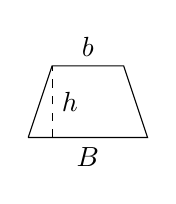
\begin{tikzpicture}[baseline=(current bounding box.center),scale=\tikzsize]
                \coordinate (A) at (0,0);
                \coordinate (B) at (1,3);
                \coordinate (C) at (4,3);
                \coordinate (D) at (5,0);
                \coordinate (H) at (1,0);
                \draw (A)-- (B) -- node[above] {$b$} (C) -- (D) -- node[below] {$B$} (A);
                \draw[dashed] (H) -- node[right]{$h$} (B);
                \addvmargin{2mm};
            \end{tikzpicture} & $\displaystyle \frac{(b+B)\cdot h}{2}$  &  
            $b+B+2\sqrt{h^2+\left( \frac{B-b}{2} \right)^2}$      \\ \hline
            Círculo &
            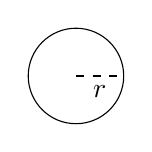
\begin{tikzpicture}[baseline=(current bounding box.center),scale=\tikzsize]
                \coordinate (A) at (2,2);
                \coordinate (B) at (4,2);
                \draw[dashed] (A)--node[below] {$r$}(B) ;
                \draw (A) circle (2cm);
                \addvmargin{2mm};
            \end{tikzpicture} & $\pi\cdot r^2$ & $2\pi\cdot r$ \\ \hline 
            Elipse &
            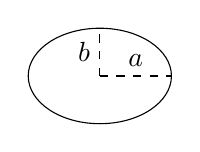
\begin{tikzpicture}[baseline=(current bounding box.center),scale=\tikzsize]
                \draw[dashed] (2,4) -- node[above] {$a$}(5,4);
                \draw[dashed] (2,4) -- node[left] {$b$} (2,6);
                \draw (2,4) ellipse (3 and 2);
                \addvmargin{2mm};
            \end{tikzpicture} & $a\cdot b \cdot \pi$ & 
            \footnotemark
             \\ 
        \end{tabular}%
    }
\end{table}

\vfill
\footnotetext{Não existe fórmula para descrever o perímetro de uma elipse.}


\pagebreak

\begin{multicols*}{2}

    \section*{Funções trigonométricas}
    As funções trigonométricas são funções que relacionam diversas propriedades
    da geometria, notoriamente as propriedades dos triângulos. Partindo do
    princípio que polígonos de mais arestas podem ser decompostos em triângulos,
    então as funções trigonométricas podem facilmente serem correlacionadas com
    demais formas geométricas não curvilíneas.

    \subsection*{o círculo trigonométrico}
    O círculo trigonométrico é um conceito que apresenta visualmente a relação
    entre as funções trigonométricas \textit{seno e cosseno} e o triângulo retângulo.
    Mas antes vamos relembrar algumas denominações relacionadas aos triângulos.

    Dado o triângulo retângulo $ABC$ abaixo:
    \begin{figure}[H]
        \centering
        %\resizebox{\columnwidth}{!}{%
        \begin{tikzpicture}
            \coordinate (A) at (0,0);
            \coordinate (B) at (4,3);
            \coordinate (C) at (4,0);
            % \coordinate (D) at (0,3);
            \node[circle, fill, label={left:$A$}, inner sep=2pt] at (A) {};
            \node[circle, fill, label={right:$B$}, inner sep=2pt] at (B) {};
            \node[circle, fill, label={right:$C$}, inner sep=2pt] at (C) {};
            % \node[circle, fill, label={left:$D$}, inner sep=2pt] at (D) {};
            % \draw[dashed] (A)--(D)--(B);
            \draw (A)-- node[above left] {$hip$} (B);
            \draw (B)-- node[right] {$CO$} (C);
            \draw (C)-- node[below] {$CA$} (A);
            \pic ["$\theta$", draw, -,angle eccentricity=2] {angle = C--A--B};
            \tkzMarkRightAngle[size=.3](A,C,B);
        \end{tikzpicture}
        %}
        \caption{Triângulo retângulo $ABC$}
        \label{fig:tri_abc}
    \end{figure}
    \noindent a aresta $\overline{AB}$ é denominada hipotenusa ou abreviadamente $hip$,
    a aresta $\overline{BC}$ é denominada cateto oposto ou $CO$ e a aresta
    $\overline{AC}$ é denominada cateto adjacente ou $CA$ pois o mesmo é
    adjacente ao ângulo $\theta$. Voltando ao círculo trigonométrico, imagine
    um círculo de raio unitário $r=1$ com origem em (0,0) cuja sombra da semirreta do raio sobre o eixo
    $x$ forme o triângulo $ABC$ conforme a fígura \ref{fig:circ_trig}.

    \begin{figure}[H]
        \centering
        % \resizebox{\columnwidth}{!}{%
        \begin{tikzpicture}
            \coordinate (A) at (0,0);
            \coordinate (IX) at (-2.5,0);
            \coordinate (FX) at (2.5,0);
            \coordinate (IY) at (0,-2.5);
            \coordinate (FY) at (0,2.5);
            \coordinate (B) at (1.5,2);
            \coordinate (C) at (1.5,0);
            \draw (IX) -- (FX)  node[right] {$x$};
            \draw (IY) -- (FY)  node[above] {$y$};
            \draw (A) node[below left] {$A$} -- (B);
            \draw (B) node[above right] {$B$} -- (C);
            \draw (C) node[below right] {$C$} -- (A);
            \draw (A) circle (2.5cm);
            \pic ["$\theta$", draw, -,angle eccentricity=2] {angle = C--A--B};
        \end{tikzpicture}
        % }
        \caption{Círculo trigonométrico}
        \label{fig:circ_trig}
    \end{figure}

    Agora, imagine que o vértice $B$ rotaciona sobre a circunferência, portanto
    a reta $\overline{AB}$ acompanha o vértice $B$ formando um movimento que se assemelha
    ao ponteiro de um relógio. Com esse exercício de imaginação é possível notar
    que o ângulo $\theta$ muda conforme a reta $AB$ rotaciona, bem como o
    comprimento de $\overline{AC}$ e $\overline{BC}$

    Começando com o ângulo $\theta=0$ e traçando o comprimento da aresta $\overline{AC}$
    ao longo do eixo $x$ até $\theta=2\pi$ obtemos o seguinte gráfico:

    \begin{figure}[H]
        \centering
        \begin{tikzpicture}
            \begin{axis}[
                    ymin=-2,
                    ymax=2,
                    trig format plots=rad,
                    axis lines = middle,
                ]
                \addplot[domain=0:2*pi,samples=200] {cos(x)};
            \end{axis}
        \end{tikzpicture}
        % \caption{Função cosseno}
        % \label{fig:circ_trig}
    \end{figure}


    Por coincidência esse gráfico é a representação da função cosseno,
    e nesse caso podemos observar que a função cosseno também representa o
    comprimento do cateto adjacente em função do ângulo $\theta$, é possível
    então deduzir que $CA = cos(\theta)$, porém essa dedução está incompleta,
    pois só abrange o caso onde $hip = 1$.

    Podemos também traçar o comprimento da aresta $\overline{BC}$ (cateto oposto)
    ao longo do eixo $x$ e obteremos um gráfico similar:
    \begin{figure}[H]
        \centering
        \begin{tikzpicture}
            \begin{axis}[
                    ymin=-2,
                    ymax=2,
                    trig format plots=rad,
                    axis lines = middle,
                    % yticklabels={$-2$,$-2$,$-r$,,$r$}
                ]
                \addplot[domain=0:2*pi,samples=200] {sin(x)};
            \end{axis}
        \end{tikzpicture}
    \end{figure}

    No caso esse gráfico é a representação da função seno, e novamente poderíamos
    deduzir que $CO = sen(\theta)$, porém novamente essa dedução estaria correta
    apenas para $hip = 1$. Para obter uma equivalência geral que descreva o
    as dimensões do triângulo retângulo utilizando as funções trigonométricas
    podemos mudar o raio do círculo trigonométrico para um $r$ qualquer,
    e nesse caso obtemos os seguintes gráficos:

    \begin{figure}[H]
        \centering
        \begin{tikzpicture}
            \begin{axis}[
                    ymin=-2,
                    ymax=2,
                    trig format plots=rad,
                    axis lines = middle,
                    yticklabels={,,$-r$,,$r$}
                ]
                \addplot[domain=0:2*pi,samples=200] {cos(x)};
            \end{axis}
        \end{tikzpicture}
        \caption{Função cosseno com amplitude $r$}
    \end{figure}

    \begin{figure}[H]
        \centering
        \begin{tikzpicture}
            \begin{axis}[
                    ymin=-2,
                    ymax=2,
                    trig format plots=rad,
                    axis lines = middle,
                    yticklabels={,,$-r$,,$r$}
                ]
                \addplot[domain=0:2*pi,samples=200] {sin(x)};
            \end{axis}
        \end{tikzpicture}
        \caption{Função seno com amplitude $r$}
    \end{figure}

    A forma da onda é a mesma do cosseno e seno, respectivamente, porém a
    amplitude agora passou a ser $r$. Voltando a tentar deduzir uma fórmula para
    o comprimento do cateto oposto e o cateto adjacente temos que:

    \begin{align}
        CO & = r\cdot sen(\theta) \\
        CA & = r\cdot cos(\theta)
    \end{align}

    \noindent sabendo que $r=hip$ temos então:
    \begin{align}
        sen(\theta)                & = \frac{CO}{hip} \label{eq:eq1} \\[1ex]
        \text{e \quad} cos(\theta) & = \frac{CA}{hip} \label{eq:eq2}
    \end{align}

    A relação da função tangente e o triângulo retângulo é difícil de ser
    explicada através do círculo trigonométrico sem o auxilio de animações visuais,
    porém podemos chegar numa relação através da igualdade conhecida onde:

    \begin{align*}
        tg(\theta) = \frac{sen(\theta)}{cos(\theta)}
    \end{align*}

    \noindent substituindo $sen(\theta)$ e $cos(\theta)$ pelas equações
    \eqref{eq:eq1} e \eqref{eq:eq2} respectivamente, temos:

    \begin{align}
        tg(\theta) & = \frac{CO}{hip}\cdot\frac{hip}{CA}                   \\[1ex]
        tg(\theta) & = \frac{CO}{\cancel{hip}}\cdot\frac{\cancel{hip}}{CA} \\[1ex]
        tg(\theta) & = \frac{CO}{CA}
    \end{align}

    Por fim temos as três equações que descrevem as razões trigonométricas de um
    triângulo retângulo:

    \begin{align}
        sen(\theta) & = \frac{CO}{hip} \\[1ex]
        cos(\theta) & = \frac{CA}{hip} \\[1ex]
        tg(\theta)  & = \frac{CO}{CA}
    \end{align}

    \begin{figure}[H]
        \centering
        \begin{tikzpicture}
            \begin{axis}[
                    ymin=-2,
                    ymax=2,
                    trig format plots=rad,
                    axis lines = middle,
                    % yticklabels={,,$-r$,,$r$}
                ]
                \addplot[domain=-1.5:1.5,samples=200] {tan(x)};
            \end{axis}
        \end{tikzpicture}
        \caption{Gráfico da função tangente}
    \end{figure}

    Devido a complexidade em se cálcular o resultado das funções trigonométricas
    seno, cosseno e tangente, muitos exercícios que envolvem essas funções acabam
    por usar valores bem conhecidos, ou valores tabelados, isso é verdade
    principalmente para os vestibulares.

    \begin{table}[H]
        % \setlength\extrarowheight{1cm}
        \renewcommand\arraystretch{2.5}
        % \newcolumntype{C}{>{$\displaystyle}c<{$}}
        \centering
        \resizebox{\columnwidth}{!}{%
            \begin{tabular}{c|c|c|c}
                    & 30° $\displaystyle \left(\frac{\pi}{6}\right)$                      & 45° $\displaystyle \left(\frac{\pi}{4}\right)$                      & 60° $\displaystyle \left(\frac{\pi}{3}\right)$                       \\ \hline
                sen & $\displaystyle \frac{1}{2}$        & $\displaystyle \frac{\sqrt{2}}{2}$ & $\displaystyle \frac{\sqrt{3}}{2}$ \\ \hline
                cos & $\displaystyle \frac{\sqrt{3}}{2}$ & $\displaystyle \frac{\sqrt{2}}{2}$ & $\displaystyle \frac{1}{2}$        \\ \hline
                tg  & $\displaystyle \frac{\sqrt{3}}{3}$ & $1$                                & $\sqrt{3}$
            \end{tabular}%
        }
        \caption{Tabela de ângulos notáveis}
        \label{tab:trig_val}
    \end{table}
 
    \subsection*{Teorema de Pitágoras}
    
    O teorema de Pitágoras é uma relação importante entre o comprimento das arestas 
    de um triângulo retângulo, sendo fundamental em muitos exercícios de geometria
    e frequentemente tópico necessário para o desenvolvimento de questões de 
    vestibular.

    \noindent
    Dado o triângulo retângulo abaixo:
    \begin{figure}[H]
        \centering
        %\resizebox{\columnwidth}{!}
        \caption{Triângulo retângulo}
        \label{fig:tri_abc}
    \end{figure}

    % \noindent 
    O teorema de Pitágoras diz que: \textit{"Em qualquer triângulo retângulo, o quadrado do comprimento da hipotenusa é 
    igual à soma dos quadrados dos comprimentos dos catetos."}, traduzindo para 
    a forma matemática: 
    \begin{align}
        a^2 &= b^2 + c^2
    \end{align}



    \subsection*{Exercícios}

    \noindent
    \execnum (ENEM 2019) Construir figuras de diversos tipos, apenas dobrando e cortando papel, 
    sem cola e sem tesoura, é a arte do origami (ori = dobrar; kami = papel), 
    que tem um significado altamente simbólico no Japão. A base do origami é o 
    conhecimento do mundo por base do tato. Uma jovem resolveu construir um
    cisne usando a técnica do origami, utilizando uma folha de papel de 18 cm 
    por 12 cm. Assim, começou por dobrar a folha conforme a figura:

    \begin{figure}[H]
        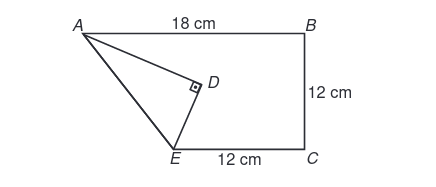
\includegraphics[width=\columnwidth]{assets/enem2019-171.png}
    \end{figure}

    \noindent 
    Após  essa  primeira  dobradura,  a  medida  do  segmento $\overline{AE}$ é:
    \begin{enumerate}[(a)]
        \item $2\sqrt{22}cm$
        \item $6\sqrt{3}cm$
        \item $12cm$
        \item $6\sqrt{5}cm$
        \item $12\sqrt{2}cm$
    \end{enumerate}

    \noindent \textbf{Solução:} 
    Esse é um simples problema que pode ser resolvido com o teorema de Pitágoras.
    Sabe-se que o triângulo $ADE$ é resultado da dobra de uma folha de papel retângular
    de $18 cm$ por $12 cm$, observando pode-se notar que a aresta (ou segmento) 
    $\overline{AD}$ tem comprimento $12cm$, e o comprimento da segmento $\overline{DE}$
    é $18-12 cm = 6cm$. Portanto, segundo o teorema de Pitágoras o segmento 
    $\overline{AE}$ é:
    \begin{align}
        \overline{AE}^2 &= \overline{AD}^2 + \overline{DE}^2\\
        \overline{AE}^2 &= 12^2 + 6^2\\
        \overline{AE} &= \sqrt{12^2+6^2}\\
        \overline{AE} &= \sqrt{180}
    \end{align}
    
    \noindent fatorando $180$ temos:
    \begin{align}
        \overline{AE} &= \sqrt{2^2\cdot 3^2\cdot 5}\\
        \overline{AE} &= 6\sqrt{5}
    \end{align}

    \noindent Portando a resposta correta é \\\textbf{d)} $\mathbf{6\sqrt{5}cm}$.\\


    \noindent 
    \execnum (ENEM 2019) Uma administração municipal encomendou a pintura
    de dez placas de sinalização para colocar em seu pátio
    de estacionamento.
    O profissional contratado para o serviço inicial
    pintará o fundo de dez placas e cobrará um valor de
    acordo com a área total dessas placas. O formato
    de cada placa é um círculo de diâmetro $d = 40 cm$,
    que tangencia lados de um retângulo, sendo que
    o comprimento total da placa é $h = 60 cm$, conforme
    ilustrado na figura. Use $3,14$ como aproximação para $\pi$.

    \begin{figure}[H]
        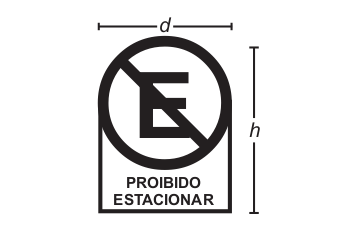
\includegraphics[width=\columnwidth]{assets/enem2019-151.png}
    \end{figure}

    \noindent
    Qual é a soma das medidas das áreas, em centímetros quadrados, das dez placas?
    \begin{enumerate}[(a)]
        \item 16.628
        \item 22.280
        \item 28.560
        \item 41.120
        \item 66.240
    \end{enumerate}

    \noindent \textbf{Solução:}
    Analisando o problema, podemos redesenhar a placa usando duas formas
    geométricas, um retângulo de lados $d$ e $h'$ e uma circunferência de 
    diâmetro $d$.
    \begin{figure}[H]
    \centering
    % \resizebox{0.5\columnwidth}{!}{%
        \begin{tikzpicture}[scale=\columnwidth/10cm]
            \coordinate (I) at (-1,0);
            \coordinate (F) at (-1,6);
            \coordinate (A) at (0,4);
            \coordinate (B) at (4,4);
            \coordinate (C) at (4,0);
            \coordinate (D) at (0,0);
            \draw[dashed] (A)-- node[above] {$d$} (B) ;
            \draw (B)-- node[right] {$h'$} (C) ;
            \draw (C)--(D)--(A);
            \draw [<->] (I)-- node[left] {$h$} (F);
            % \draw (2,4) -- node[above] {$r$}(C); 
            % \draw[dashed] (2,0)-- node[left] {$h$}(2,4) ;
            % \draw (2,4) ellipse (2 and 1);
            \draw (B) arc(0:180:2 and 2);
            \draw[dashed] (A) arc(180:360:2 and 2);
        \end{tikzpicture}
    % }
    % \caption{Cilindro}
    \end{figure}

    \noindent A área da placa pode ser obtida com a soma da área do retângulo 
    com a metade da área da circunferência, mas para calcularmos a área do 
    retângulo devemos calcular o comprimento $h'$ que nada mais é que $h-\frac{d}{2}$, 
    portanto $h' = 40cm$, resolvendo:
    \begin{align}
        A_{placa} &= \frac{A_{circ}}{2} + A_{ret}\\[1ex]
        A_{circ} &= \pi\left( \frac{d}{2} \right)^2 = 1256cm^2\\
        A_{ret} &= h'\cdot d = 1600cm^2 \\
        A_{placa} &= \frac{1256}{2} + 1600 = 2228 cm^2
    \end{align}
    \noindent Como o exercício pede a área total das dez placas, é só 
    multiplicarmos a área de uma placa por dez e temos $22280cm^2$, portanto a 
    alternativa correta é \textbf{b) 22.280}\\

    \execnum (ENEM 2017) Um caminhão de grande porte entalou embaixo do viaduto no 
    cruzamento das avenidas Borges de Medeiros e Loureiro da silva no sentido 
    Centro-Bairro, próximo á Ponte de Pedra, na capital. Esse veículo vinha de 
    São Paulo para Porto Alegre e transportava três grandes tubos, conforme
     ilustrado na foto.  

     \begin{figure}[H]
        \centering
        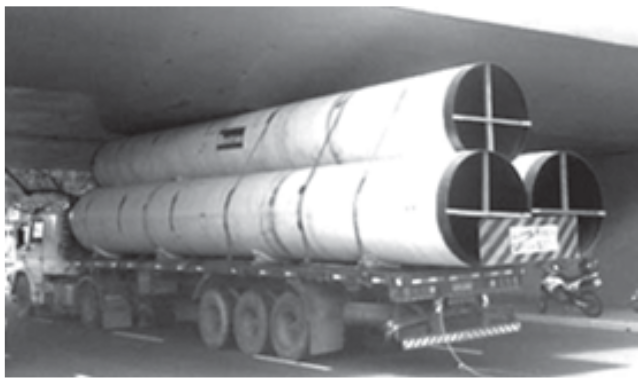
\includegraphics[width=0.75\columnwidth]{assets/enem2017-157.png}
        % \caption{Disponível em: www.caminhoes-e-carretas.com. Acesso em: 21 maio 2012 (adaptado).}
    \end{figure}

    Considere que o raio externo de cada cano da imagem seja $0,60m$ e que eles 
    estejam em cima de uma carroceria cuja parte superior está a $1,30m$ do solo.
    O desenho representa a vista traseira do empilhamento dos canos.
    
    \begin{figure}[H]
        \centering
        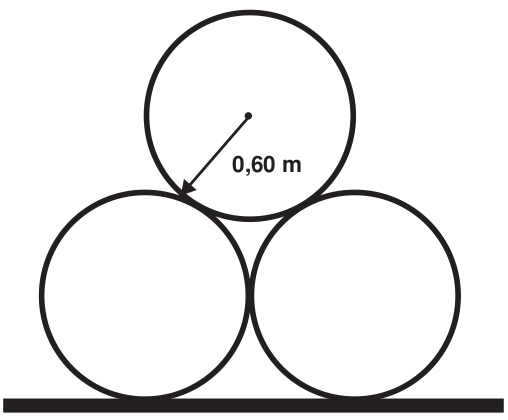
\includegraphics[width=0.75\columnwidth]{assets/enem2017-157-2.png}
    \end{figure}

    A margem de segurança recomendada para que um veículo passe sob um viaduto é que
    a altura total do veículo com a carga seja, no mínimo, $0,50m$ menor do que a altura
    do vão do viaduto.
    Considere $1,7$ como aproximação para $\sqrt{3}$.
    Qual deveria ser a altura mínima do viaduto, em metro, para que esse caminhão 
    pudesse passar com segurança sob seu vão?
    \begin{enumerate}[(a)]
        \item 2,82
        \item 3,52
        \item 3,70
        \item 4,02
        \item 4,20
    \end{enumerate}

    \textbf{Solução:} Em resumo o problema pede a altura da pilha de tubos, 
    acrescido da altura da carroceria do caminhão ($1,30m$) e a margem de segurança ($0,50m$).
    Considerando que a altura da pilha de tubos seja $x$, portanto a resposta é 
    $x+1,80m$. Basta portanto encontrarmos a altura da pilha de tubos, e analisando 
    o problema temos o seguinte: 
    
    \begin{figure}[H]
        \centering
        % \adjustbox{width=0.8\columnwidth}{
            \begin{tikzpicture}[scale=\columnwidth/10cm]
                \coordinate (A) at (0,0);
                \coordinate (B) at (2,3.5);
                \coordinate (C) at (2,0);
                \draw (A) circle (2 and 2);
                \draw (B) circle (2 and 2);
                \draw (4,0) circle (2 and 2);
                \draw[<->] (-2.3,-2) -- node[left] {$x$} (-2.3,5.4);
                \draw[<->] (-3,-2) -- node[left] {$r$}  (-3,0);
                \draw[<->] (-3,0) -- node[left] {$h$}   (-3,3.5);
                \draw[<->] (-3,3.5) -- node[left] {$r$} (-3,5.4);
                \draw[dashed] (A)-- node[below left] {$1,2m$}(B);
                \draw[dashed] (B)-- node[above right] {$h$} (C)-- node[below] {$0,6m$}(A);
                \pic ["$60^{\circ}$", draw, -, angle eccentricity=2] {angle = C--A--B};
                % \tkzMarkRightAngle[size=.3](A,C,B);
            \end{tikzpicture}
        % }
        % \caption{Cilindro}
    \end{figure}

    Perceba que entre o centro das circunferências podemos formar um triângulo 
    equilátero que pode ser então dividido em dois triângulos retângulos de arestas 
    $1,20m$, $0,60m$ e $h$. A altura total $x$ é composta por $h + 2r$, onde 
    o $r$ se refere ao raio do círculo $0,60m$, e a resposta final 
    pode ser reescrita como $h+3m$. Para encontrar o $h$ devemos 
    lembrar da relação entre as funções trigonométricas e os triângulos retângulos
    e como $h$ é o cateto oposto ao ângulo $60^\circ$ temos que:
    \begin{align}
        sen(60^\circ) &= \frac{h}{1,20m} \label{eq1:enem3}
    \end{align}
    Consultando a tabela \ref{tab:trig_val}, temos que $sen(60^\circ) = \sqrt{3}/2$
    , portanto da equação \ref{eq1:enem3} temos:  
    
    \begin{align}
        \frac{\sqrt{3}}{2} &= \frac{h}{1,20m}\\
        h &= 1,2\cdot\frac{\sqrt{3}}{2}\\
        h &= 1,02
    \end{align}
    
    Logo, a resposta final dada por $h+3m$ resulta em $4,02m$. Portanto a resposta
    correta é \textbf{d) 4,02}. É possível calcular o valor de $h$ usando o 
    teorema de Pitágoras, porém caímos numa raiz quadrada que é difícil de calcular
    sem o auxílio de yma calculadora.\\
    
    \execnum (UNICAMP 2016) Um cilindro circular reto, cuja altura é igual ao diâmetro da 
    base, está inscrito numa esfera. A razão entre os volumes 
    da esfera e do cilindro é igual a:
    \begin{enumerate}[(a)]
        \item $4\sqrt{2}/3$
        \item $4/3$
        \item $3\sqrt{2}/4$
        \item $\sqrt{2}$
    \end{enumerate}

    \textbf{Solução:} O problema não especifica o raio da esfera nem da base do cilindro, porém 
    ele nos informa que o cilindro está inscrito na esfera e que a altura do cilindro é 
    a mesma do diâmetro da base, portanto analisando o problema chegamos na seguinte representação gráfica:

    \begin{figure}[H]
        \centering
        \resizebox{0.5\columnwidth}{!}{%
            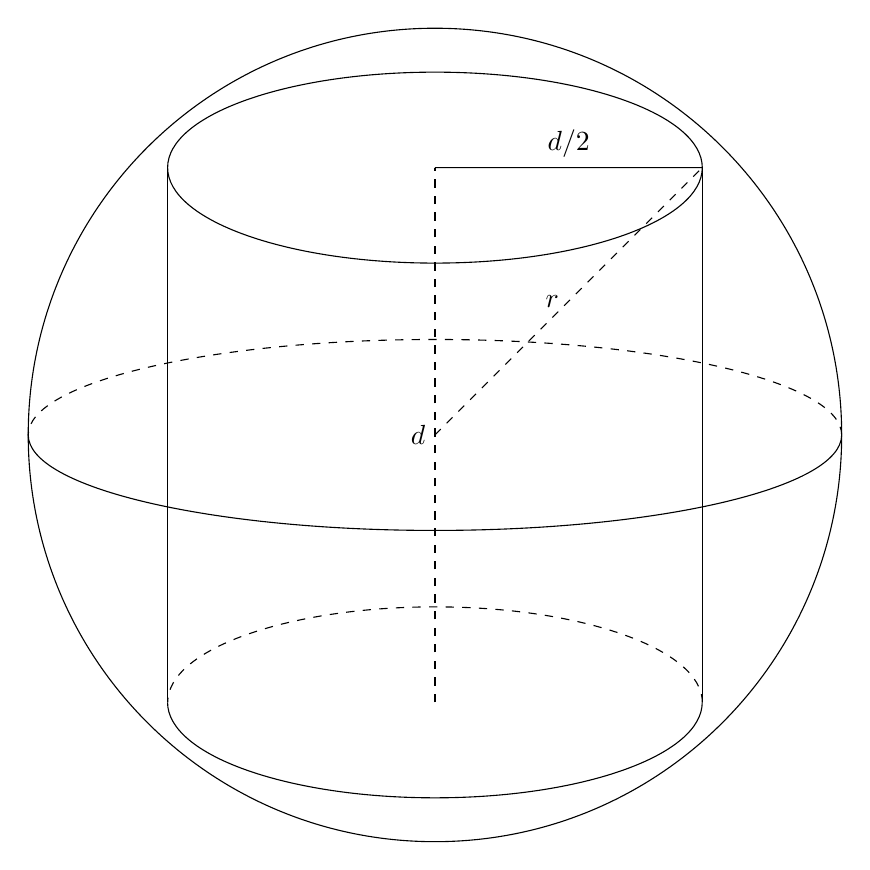
\begin{tikzpicture}[scale=\columnwidth/10cm]
                \coordinate (A) at (-2.8,-2.8);
                \coordinate (B) at (-2.8,2.8);
                \coordinate (C) at (2.8,2.8);
                \coordinate (D) at (2.8,-2.8);
                %circulo
                \draw (-4.26,0) arc (180:360:4.26 and 1);
                \draw[dashed] (4.26,0) arc (0:180:4.26 and 1);
                \draw[dashed] (D) arc(0:180:2.8 and 1);
                \draw (0,0) circle (4.26 and 4.26);
                %cilindro
                \draw (A)--(B) ;
                \draw (C)--(D) ;
                \draw (0,2.8) -- node[above] {$d/2$}(C); 
                \draw[dashed] (0,-2.8)-- node[left] {$d$}(0,2.8) ;
                \coordinate (A1) at (0,0);
                \coordinate (B1) at (2,0);
                \draw (0,2.8) ellipse (2.8 and 1);
                \draw (A) arc(180:360:2.8 and 1); 
                \draw[dashed] (0,0) -- node[left]{$r$}(C);
                % \draw (0,2) arc (90:270:1 and 2);
                % \draw[dashed] (0,-2) arc (-90:90:1 and 2);
                % \draw (A1)-- node[above] {$r$} (B1);
            \end{tikzpicture}
        }
        \caption{Cilíndro}
    \end{figure}

    O volume do cilindro é facilmente calculável dado um diâmetro $d$ arbitrário, 
    porém não possuímos o raio da esfera, na qual devemos obter com os parâmetros 
    que já temos. Note que se traçarmos uma reta do centro do cilindro até a circunferência da base do 
    cilindro temos então uma reta cujo comprimento coincide com o raio da esfera, 
    além disso formamos um triângulo isósceles e retângulo com arestas $d/2$, $d/2$ e $r$.
    

    \begin{figure}[H]
        \centering
        % \adjustbox{width=0.8\columnwidth}{
            \begin{tikzpicture}[scale=\columnwidth/10cm]
                \coordinate (A) at (0,0);
                \coordinate (B) at (0,4);
                \coordinate (C) at (4,4);
                \draw (A)-- node[left] {$d/2$}(B);
                \draw (B)-- node[above] {$d/2$}(C);
                \draw (C)--node[below right] {$r$}(A);
                \tkzMarkRightAngle[size=.3](A,B,C);
            \end{tikzpicture}
        % }
        % \caption{Cilindro}
    \end{figure}

    Logo, utilizando o teorema de Pitágoras obtemos que o raio é:
    \begin{align}
        r^2 &= \left(\frac{d}{2}\right)^2+\left(\frac{d}{2}\right)^2\\[1ex]
        r^2 &= \frac{d^2}{2}\\[1ex]
        r &= \frac{d}{\sqrt{2}}
    \end{align} 

    Agora podemos calcular o volume da esfera:
    \begin{align}
        V_e &= \frac{4}{3}\pi r^3 \\[1ex]
        V_e &= \frac{4}{3}\cdot\left(\frac{d}{\sqrt{2}}\right)^3\pi
        = \frac{2d^3\pi}{3\sqrt{2}}
    \end{align}
    E o volume do cilindro:
    \begin{align}
        V_c &= \pi \left( \frac{d}{2} \right)^2 \cdot d\\[1ex]
        V_c &= \frac{d^3\pi}{4}
    \end{align}
    Portanto a razão entre o volume da esfera e do cilindro é:
    \begin{align}
        \frac{V_e}{V_c} &= \frac{2d^3\pi}{3\sqrt{2}}\cdot \frac{4}{d^3\pi}\\[1ex]
        \frac{V_e}{V_c} &= \frac{2\cancel{d^3\pi}}{3\sqrt{2}}\cdot \frac{4}{\cancel{d^3\pi}}\\[1ex]
        \frac{V_e}{V_c} &= \frac{8}{3\sqrt{2}}
    \end{align}
    Racionalizando:
    \begin{align}
        \frac{V_e}{V_c} &= \frac{8}{3\sqrt{2}} \cdot\frac{\sqrt{2}}{\sqrt{2}}\\
        \frac{V_e}{V_c} &= \frac{8\sqrt{2}}{3\cdot2} = \frac{4\sqrt{2}}{3}
    \end{align}

    \noindent Portanto a resposta correta é \\\textbf{a)} $\mathbf{4\sqrt{2}/3}$
    
    % \newpage
    % \subsection*{Apenas para referência}
    % \begin{figure}[H]
    %     \centering
    %     \resizebox{0.5\columnwidth}{!}{%
    %         \begin{tikzpicture}
    %             \coordinate (A) at (0,0);
    %             \coordinate (B) at (0,4);
    %             \coordinate (C) at (4,4);
    %             \coordinate (D) at (4,0);
    %             \draw (A)--(B) ;
    %             \draw (C)--(D) ;
    %             \draw (2,4) -- node[above] {$r$}(C); 
    %             \draw[dashed] (2,0)-- node[left] {$h$}(2,4) ;
    %             \draw (2,4) ellipse (2 and 1);
    %             \draw[dashed] (D) arc(0:180:2 and 1);
    %             \draw (A) arc(180:360:2 and 1);
    %         \end{tikzpicture}
    %     }
    %     \caption{Cilindro}
    % \end{figure}

    % \begin{figure}[H]
    %     \centering
    %     \resizebox{0.5\columnwidth}{!}{%
    %         \begin{tikzpicture}
    %             \coordinate (A) at (0,0);
    %             \coordinate (B) at (2,0);
    %             \draw (-2,0) arc (180:360:2 and 1);
    %             \draw[dashed] (2,0) arc (0:180:2 and 1);

    %             % \draw (0,2) arc (90:270:1 and 2);
    %             % \draw[dashed] (0,-2) arc (-90:90:1 and 2);
    %             \draw (0,0) circle (2 and 2);
    %             \draw (A)-- node[above] {$r$} (B);
    %         \end{tikzpicture}
    %     }
    %     \caption{Esfera}
    % \end{figure}

    % \begin{figure}[H]
    %     \centering
    %     %\resizebox{0.5\columnwidth}{!}{%
    %         \begin{tikzpicture}
    %             \coordinate (A) at (0,0);
    %             \coordinate (B) at (0,3);
    %             \coordinate (C) at (3,3);
    %             \coordinate (D) at (3,0);
    %             \coordinate (E) at (1,1);
    %             \coordinate (F) at (1,4);
    %             \coordinate (G) at (4,4);
    %             \coordinate (H) at (4,1);
    %             \draw (A)--(B)--(F)--(G)--node[right]{$l$}(H)--node[right]{$l$}(D)--node[below]{$l$}(A);
    %             \draw (B)--(C)--(D);
    %             \draw (C)--(G);
    %             \draw[dashed] (A)--(E)--(H);
    %             \draw[dashed] (E)--(F);
    %         \end{tikzpicture}
    %     %}
    %     \caption{Cubo}
    % \end{figure}


    % \begin{figure}[H]
    %     \centering
    %     
\includegraphics[width=0.7\columnwidth]{assets/image_placeholder.png}
    %     \caption{Tetraedro, o objeto tridimenssional com menos faces}
    % \end{figure}



\end{multicols*}